\chapter{Clean Architecture}\label{cleanArchitecture}

Zum implementieren der Clean Architecture wurde ein UML Diagramm erstellt (Abb.~\ref{Abb:CleanArchitectureBEFORE} im Anhang) um die aktuellen Abhängigkeiten zu sehen, dabei wurden ein paar Abhängigkeitspfeile weggelassen welche von weit außen nach innen gehen und die Lesbarkeit zu sehr verringern. 


Für die Struktur der Clean Architektur wurde sich auf 4 Schichten festgelegt, da die Funktionsweise des Programms recht simpel ist. Die innerste Schicht beinhaltet alle Entitäten welche zur strukturierten Datenspeicherung verwendet werden. Die mittlere hellblaue Schicht umfasst die Anwendungslogik. Die dunkelgrüne Schicht beinhaltet die Interaktion mit allem Außerhalb, d.h. die Controller zum lesen und schreiben der Daten auf der Festplatte sowie zum kommunizieren mit der GUI. Ganz außen befinden sich die Speicherorte der Spieldaten und die GUI Elemente. 


\begin{figure}[!ht]
  \centering
  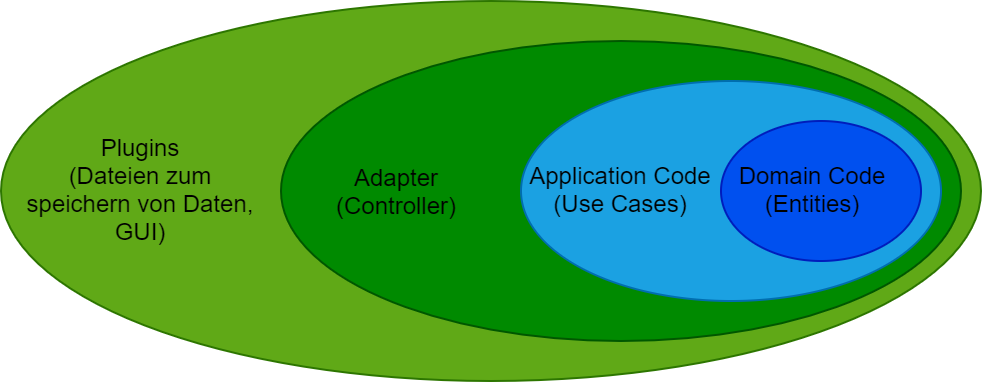
\includegraphics[width=0.6\textwidth]{Bilder/ArchitekturSchichten.PNG}
  \caption{Aufbau der Schichten der Clean Architecture in der Anwendung}
  \label{Abb:ArchitekturSchichten}
\end{figure}

\paragraph{Abhängigkeiten}
Ein großes Problem sind die Abhängigkeiten von Innen nach Außen, wie z.B. die \href{https://github.com/EinToni/Wortfinder/blob/main/Wortfinder/WordGenerator.cs}{\textit{WordFinder}} (umbenannt zu \textit{WordGenerator}) Klasse, welche direkt auf den \href{https://github.com/EinToni/Wortfinder/blob/586681478211a26abc661239ecc2c297ef77041e/Wortfinder/DataController.cs}{\textit{DataController}} zugreift, siehe.~\ref{Abb:CleanArchitectureBEFORE} auf Seite~\pageref{Abb:CleanArchitectureBEFORE}. Die Abhängigkeit wird durch Dependency Inversion, d.h. die Erstellung eines Interfaces welches von der äußeren Klasse implementiert und von der inneren genutzt wird, umgedreht. Die Dependency Inversion ist in der nachfolgenden Abbildung dargestellt und in Commit \href{https://github.com/EinToni/Wortfinder/commit/586681478211a26abc661239ecc2c297ef77041e}{586681478211a26abc661239ecc2c297ef77041e} umgesetzt.
\newpage
\begin{figure}[!ht]
  \centering
  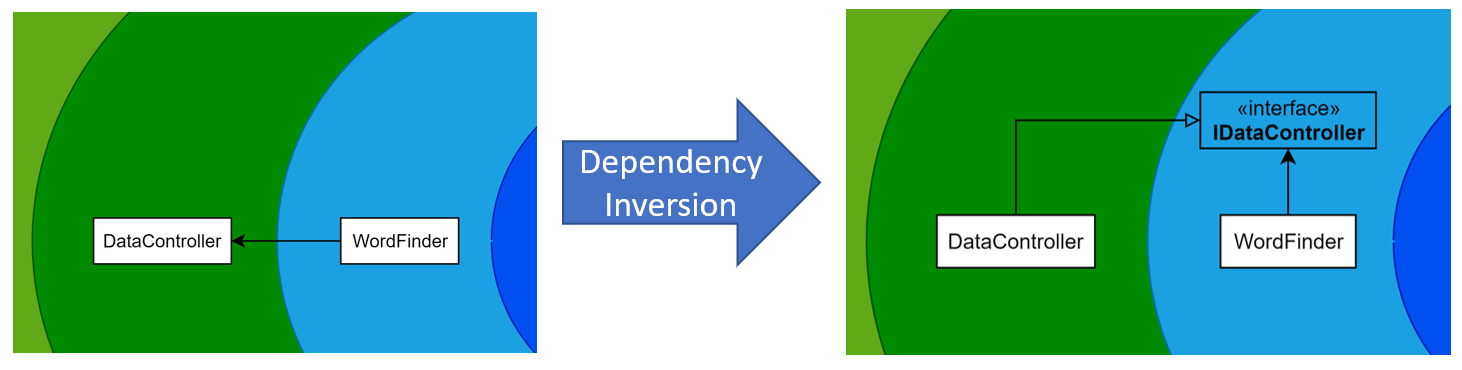
\includegraphics[width=0.8\textwidth]{Bilder/DependencyInversion.PNG}
  \caption{Beispiel der Dependency Inversion}
  \label{Abb:DependencyInversion}
\end{figure}

\paragraph{Abstrakte Fabrik}
Oftmals haben Klassen in inneren Schichten, Klassen aus äußeren Schichten instantiiert. Ein Beispiel dafür ist ebenfalls der  \textit{WordFinder}, welcher im Konstruktor eine eine Instanz des \textit{DataController} erstellt hat. Unter Einhaltung der Clean Architecture geht das allerdings nicht. Da vermieden werden wollte, dass die Referenzen auf diese äußeren Klassen von der Main aus weit \glqq nach unten gereicht\grqq{} werden, wurde das Erzeugungsmuster der abstrakten Fabrik verwendet. Dem \textit{WordFinder} wird dann im Konstruktor eine Referenz auf die Fabrik gegeben. Über die Funktion \glqq GetDataController()\grqq{} gibt die Fabrik dann eine neue Instanz des \textit{DataController} zurück, wobei der Rückgabetyp im Interface der Fabrik als \textit{IDataController} Deklariert ist, vgl. Commit \href{https://github.com/EinToni/Wortfinder/commit/26148d6a7ae6784b935a260371672fe16f8bbfa0}{26148d6a7ae6784b935a260371672fe16f8bbfa0}:

\begin{figure}[!ht]
  \centering
  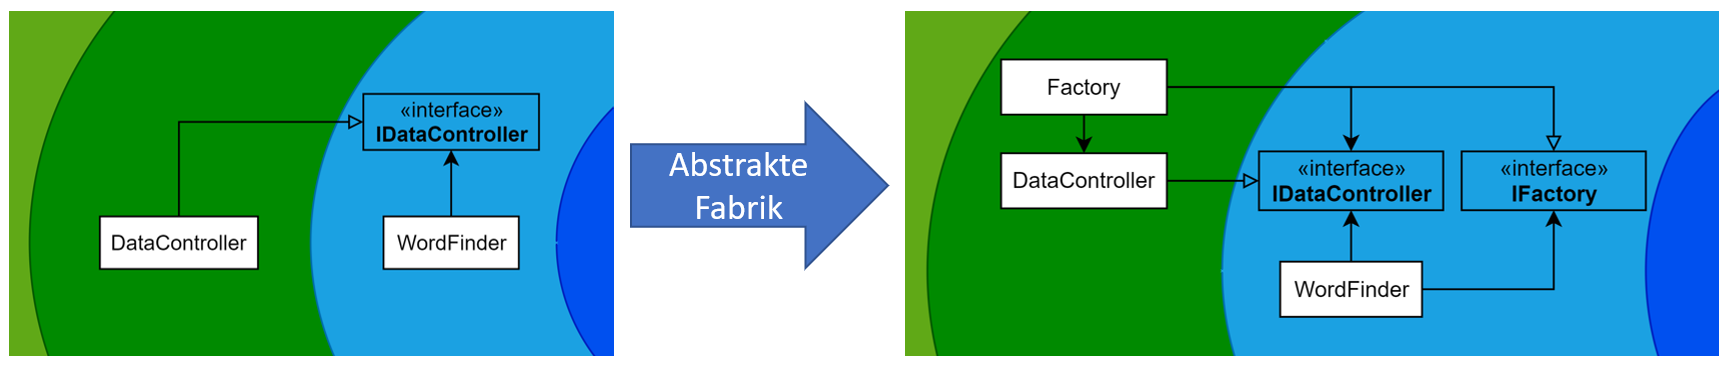
\includegraphics[width=0.8\textwidth]{Bilder/AbstrakteFabrik.PNG}
  \caption{Implementierung der abstrakten Fabrik}
  \label{Abb:AbstrakteFabrik}
\end{figure}

\paragraph{Separierung der GUI}
Außerdem problematisch ist der grundsätzliche Aufbau des Programms, sowie speziell der Aufbau des Hauptfensters. Dieses bestand aus einem Grid welches durch den \textit{FieldGenerator} mit Teilfenstern (\textit{LetterBox}, zeigen die Buchstaben an) gefüllt wurde. Jeder \textit{LetterBox} wurde die Instanz des \textit{WordBuilder} gegeben, welchen sie aufrufen wenn sie angeklickt werden.


Zur Verbesserung der Trennung zwischen dem Application Code und der GUI, wird das Grid direkt im Code Behind des \textit{MainWindow} mit WPF  Elementen aufgebaut. Die Ansteuerung des \textit{MainWindow} erfolgt dann über einen neuen \textit{MainWindowController} dem im Aufruf nur die Größe des Spielfelds und die Buchstaben übergeben werden. Somit erfolgt die Erstellung der GUI separiert vom restlichen Anwendungscode.

\paragraph{Umsetzung}
Vor der eigentlichen Implementierung wurde zuerst das erstellte UML Diagramm abgeändert. Zuerst wurde dabei die Struktur geändert, sodass alle Klassen an ihrem sinnvollsten Ort sind. Dann wurden alle Abhängigkeitspfeile welche nach außen zeigen mittels Dependency Inversion umgedreht und als letztes an notwendigen Stellen eine Abstrakte Fabrik hinzugefügt. 

Da die Anwendung vorher immer nur mit Funktionen ergänzt wurde und dabei lediglich Wert auf Funktionalität gelegt wurde, sind einige unnötig komplexe Strukturen entstanden. Diese wurde daher ebenfalls direkt geändert.
Ein Beispiel hierfür ist die \textit{FindableWords} Klasse, welche alle im aktuelle laufenden Spiel findbaren Wörter beinhaltet. Diese wurde erst später hinzugefügt, da davor direkt jedes vom Nutzer markierte Wort im heruntergeladenen Wörterbuch überprüft wurde. Sowie die \textit{GameGrid} Klasse, welche (unter anderem) die Größe und Buchstaben des Spielfelds beinhaltet. Die findbaren Wörter sowie die Buchstaben im aktuellen Spiel wurden in eine neue Klasse \textit{Game} verschoben welche alle Daten über Spiel enthält. Dies ermöglicht das generieren im Vorhinein anschließende und speichern von Spielen.

Das daraus entstandene Diagramm ist im Anhang als Abbildung~\ref{Abb:CleanArchitectureAFTER}.


\paragraph{Klassen Instantiierung}
Manche Klassenreferenzen werden trotz der Abstrakten Fabrik teilweise immer noch sehr weit an nachfolgende Klassen \glqq weitergereicht\grqq, was sehr unschön ist. Daher wurde die Erstellung aller Klassen und deren Dependency Injection in die Main verschoben. Dadurch wird das unschöne und unübersichtliche weiterreichen vermieden. Auch die Erzeugung von Klassen im Konstruktor wird durch Dependency Injection ersetzt, wodurch beim Testen ein Mock-Objekt an die zu testende Klasse übergeben werden kann. Außerdem können die abstrakten Fabriken hierdurch auch wieder entfernt werden, da alle Klassen direkt in der Main erzeugt werden und von den betroffenen Klassen nur eine Instanz benötigt wird. Der Commit in welchem alle Initialisierungen in die Main ausgelagert wurde und somit die Implementierung der Clean Architecture abgeschlossen ist, ist: \href{https://github.com/EinToni/Wortfinder/commit/15e467c93903dac44e916c61f76792d385abd087}{15e467c93903dac44e916c61f76792d385abd087}. Das sich hieraus ergebende Klassendiagramm ist im Anhang~\ref{Abb:CleanArchitectureAFTERinMain}.


\paragraph{Nachträgliche Korrektur}
Nicht eingehalten wurde die Clean Architecture bei der \textit{WebScraper} und \textit{WordMissingWindow} Klasse. Die beiden Klassen wurden dabei direkt aus dem Controller des \textit{MainWindow}s aufgerufen. Denn zum Zeitpunkt des Commits war geplant diese nicht mehr zu verwenden und später zu entfernen. Da sie allerdings in Zukunft doch noch verwendet werden sollen, wurden sie, sowie weitere zugehörige Klassen, im Nachhinein korrekt angepasst. Das Klassendiagramm nach welchem die Implementierung durchgeführt wurde ist nachfolgend abgebildet. Zu beachten ist allerdings, dass nur die Struktur und die GUI implementiert wurden. Für die korrekte Funktionalität des WebScrapers fehlte leider die Zeit. Diese soll aber in Zukunft online im Duden das als fehlend angegebene Wort nachschlagen und prüfen ob es existiert. Commit der Implementierung: \href{https://github.com/EinToni/Wortfinder/commit/163a14f0730bb69c9805b4ee0421e415ce8c897d}{163a14f0730bb69c9805b4ee0421e415ce8c897d}

\begin{figure}[htb]
\centering
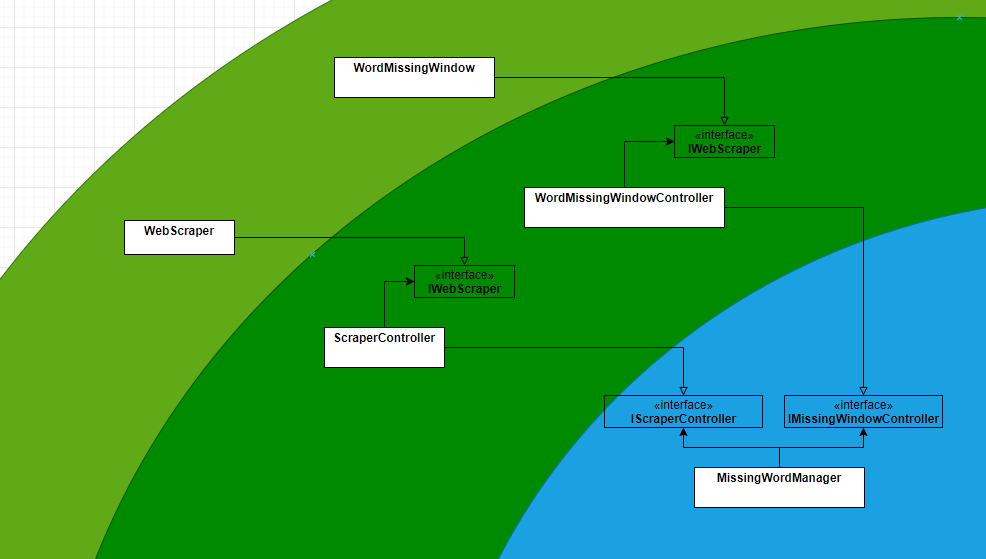
\includegraphics[width=0.8\textwidth]{Bilder/CleanArchitectureWebScraper.PNG}
\caption{\label{Abb:CleanArchitectureWebScraper}Vereinfachtes Klassendiagramm des WebScrapers und zugehöriger GUI}
\end{figure}

\endinput